OGGM-Edu (\href{http://edu.oggm.org}{http://edu.oggm.org}) is an educational website about glaciers.

I briefly summarize its main goals and history here: the interested reader is invited to have a look at
\href{https://edu.oggm.org}{the platform itself} to explore its content!

\begin{figure}[h]
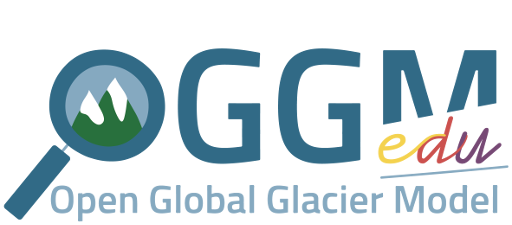
\includegraphics[width=0.4\linewidth]{\figs/oggm_edu_s_alpha.png}
\end{figure}


\section{Concept}

OGGM-Edu’s main goal is to provide interactive tools and materials for instructors who want to
teach about glaciers and glacier modelling at school, in workshops or at the university.
It does not provide much fundamental textbook material, unless at places where we found it very necessary.
In general, we link to more comprehensive, additional online resources such as
\href{http://www.antarcticglaciers.org/}{AntarcticGlaciers.org} for the theoretical background.

Everything on OGGM-Edu is open-source: one can find all our content, apps, and website \href{https://github.com/OGGM/oggm-edu}{on GitHub}.
The platform is designed to be collaborative, and any interested person can contribute via GitHub with a new experiment,
a typo correction, a translation…

Finally, all OGGM-Edu tools should work in the web browser and do not require installation: instructors simply need to
make sure that students have a computer with an internet connection to get them started.


\section{Content}

OGGM-Edu offers four largely independent components that can be combined for a longer class:
\begin{itemize}[nosep]
\item {} 
\href{https://edu.oggm.org/en/latest/\#title-graphics}{Graphics}: open access images and graphics that
illustrate some basic concepts about glaciers and that can be used in lectures or presentations.
They were designed for a general audience and are a good entry point to glaciers.

\item {} 
\href{https://edu.oggm.org/en/latest/\#title-apps}{Interactive web applications}: ready to use, interactive graphics on the web.
They come with introduction materials and videos about how to use them, as well as example questions which can be explored in class.
The targeted audience is very broad, from school children to adults, with
or without scientific background.

\item {} 
\href{https://edu.oggm.org/en/latest/\#title-notebooks}{Interactive Notebooks}: \href{https://jupyter.org/}{Jupyter notebooks} that combine narrative text,
equations, executable code and visualisations in one document. They are designed for students willing to run and develop their
own experiments. The targeted audience are students at the undergrad or graduate level with some
programming experience, or under the supervision of an instructor who can show them how to run the experiments.

\item {} 
\href{https://edu.oggm.org/en/latest/oggm\_tuto.html}{OGGM tutorials}: for current and future users of the Open Global Glacier Model.

\end{itemize}


\section{Known applications in classes}

It is very difficult for us to know the extent to which OGGM-Edu is already used (or considered for use) in classes.
Feedback so far on social media or on CRYOLIST has been very positive, but we haven’t received concrete improvement suggestions
or bugfix requests either (which can be seen as a good or a bad thing).

Here are some examples of application we are aware of:
\begin{itemize}[nosep]
\item {} 
OGGM-Edu (apps, notebooks) is used as part of the practical sessions in the “Cryosphere in the Climate System”
lecture, taught in the master program “Atmospheric Sciences” at the University Innsbruck.

\item {} 
OGGM-Edu (apps + edited and translated notebooks) has benn used for a week-long workshop for undergraduate students
in Peru.

\item {} 
The OGGM-Edu apps were used in at least three university-level classes for which we received positive feedback from
the instructors themselves \href{https://twitter.com/iceclimate/status/1359280232990199809}{on social media} and per mail.

\end{itemize}


\section{Project history, funding and outlook}

The OGGM-Edu website was launched at the end of 2018. The main bulk of the website development was done by myself,
and large parts of the content has been writen by master students. I was able to hire a student (Zora Schirmeister)
early in the process thanks to  a small digital sciences grant offered by the University of Innsbruck to work on the
first notebooks.

In 2019, I applied and obtained a much larger grant from an outreach scheme of the University of Innsbruck
(“Förderkreis \textbf{1669} -- \textbf{Wissen}schafft Gesell\textbf{schaft}”, 20k\texteuro{}),
which allowed me to hire four students (Zora Schirmeister, Patrick Schmitt, Daniel Frisinghelli, Alzbeta Medvedova)
to work part-time on the project for one year. This led to the development of the four web applications,
and to the development of several new notebooks.

I also applied and obtained a 10k\texteuro{} computational resources grant from Google Cloud’s “Data Solutions for Change”
(a programme now discontinued). This grant allowed us to host the applications on controlled resources instead of free,
but unreliable ones. This allowed us to provide a “hub” (online computer resources) to Lizz Ultee’s students during
\href{https://oggm.org/2019/12/06/OGGM-Edu-AGU/}{her workshop in Peru}. Again, the main advantage of these resources
being the complete removal of the installation’s burden. At the end of this Google grant in 2020, we moved OGGM-hub
and the hosting of our applications to our own HPC facilities in Bremen.

Today, I think that the platform is useful as it is. Since 2020, the improvements to the platform have been incremental,
mostly with improvements to the interactive apps (which, we believe, are the most used tools on the platform). Further
improvements might come from the instructors themselves - for example, the “glaciers as water resources” notebook
was developed as part of Lizz Ultee’s workshop.

Like for software, the main obstacle towards further large scale developments are: funding, staff, and time.
Again, traditional funding schemes are not really appropriate for OGGM-Edu. Many funders now explicitly ask
for an outreach component (a role that OGGM-Edu could fill for OGGM related projects), and if there is
interest from project staff to invest time in OGGM-Edu’s development, it is likely to continue to grow.

I think that the students who worked on OGGM-Edu should be very proud of what they have achieved!